\chapter{Intégration de Données Multi-Echelles et Extraction de Connaissances en Agronomie: Exemples et Perspectives \\ \vspace{0.3cm} \small{Application en Génomique Fonctionnelle chez le Riz}} % Main chapter title

\label{Perspectives} % For referencing the chapter elsewhere, use \ref{Chapter1}

This chapter draws perspectives related to my on-going research on spatio-temporal data mining.
I would discuss in which direction my research activities can evolve in the next four, five years. All the perspectives presented in this chapter are related to students I am co-supervising and projects I am involved in. %The second part of this chapter discusses medium term objectives involving more ambitious and challenging research directions and some possible idea about how these objectives can be met.


\section{Research Objectives}
In the last years, from the time I joined the TETIS laboratory, I concentrated my research efforts toward the analysis of dynamic data in which the temporal dimension plays a major role. As I discussed in the previous chapter, I studied, designed and developed, with researchers I worked with, new approaches in both pattern mining and machine learning fields to manage, in particular, the temporal dimension present in spatio-temporal databases. The complexity of such data is given by the temporal but also by the spatial information it contains. This is why, my next research objectives will focus on increasing my knowledge through the study and the development of methods that explicitly deal with spatial autocorrelation inside the data.

My research background ranges from supervised and semi-supervised machine learning methods to cluster analysis, to the design of pattern mining approaches to mine and extract knowledge from databases. 
In the current data science literature, many methods to manage spatial information already exist~\cite{BogornyS10}. 
My main objective is to design, develop and implement new approaches development of new approaches to deal with the particular kind of data I am focusing on: Time Series of Remote Sensing Data.
To pursue this goal, in the future, the next PhD fellowships I will supervised, they will be focused on the analysis of general spatio-temporal data mining techniques considering the Remote Sensing field as privilegiate domain of application.

%At the current stage, my research objectives are deeply related to the PhD students I am co-supervising.
The PhD students I am currently co-supervising, are mainly focusing on methods to mine and learn from Remote Sensing (RS) Data. Particularly, the different on-going thesis in which I am involved, they also reflect my different research backgrounds (pattern mining,  cluster analysis and supervised learning).



\section{Graph-based approaches to analyze spatial information}
\label{multigraph-mining}


General graph data mining approaches~\cite{YanH02,KuramochiK05,ElseidyASK14} traverse the search space of graph patterns and, once a pattern is generated, test its support. The algorithms can work in a transactional setting~\cite{YanH02} (the database is constituted by a collection of graphs) or extract frequent graphs in a single graph setting~\cite{KuramochiK05,ElseidyASK14} (the database is constituted by only one big graph). The most time consuming and crucial operation in such approaches is the subgraph isomorphism test~\cite{BonniciGPSF13} that allows to retrieve all the embeddings (occurrences) of a graph pattern in the graph database. 
Multigraph pattern mining seems similar to general graph mining but it has its peculiarity. The main difference relies in the subgraph isomorphism test~\cite{Ingalalli15}.
During the on-going PhD Thesis of M. Vijay Ingalalli, co-supervised in collaboration with Prof. Pascal Poncelet (LIRMM), we have developed a method to perform subgraph isomorphism test for multigraph~\cite{Ingalalli15}. The next step of this research involves the design and the implementation of a frequent multigraph mining approach. The approach will leverage techniques and tricks already proposed in the general domain of graph mining but it will introduce specific pruning strategies tailored for the multigraph structure.

In the remote sensing context we can take, as a toy example, the extraction of complex landscape interactions. Given a satellite image we can easily model the image content as a multigraph. After image segmentation, for each segment we can compute a set of characteristics induced by its radiometric attributes. This results in a vector of numerical features. The set of segments is the set of the nodes of the multigraph and two nodes are linked each other if they are spatially adjacent. More in detail, we can have a different edge type for each of the segment's feature. In this way, an edge of type $t_i$ exists between two objects if they are spatially adjacent and they have similar values w.r.t. feature $f_i$. An example of this process is reported in Figure~\ref{fig:multigraphExample} where, for the sake of clarity, a geographical area is segmented, numerical features are computed and the mulitgraph is built following the previous strategy. Different edge types are represented by different colors.

\begin{figure}[!ht]
\begin{center}
	\includegraphics[width=0.70\textwidth]{Figures/bpa_multi_layer.png}
\end{center}
\caption{Example of multigraph representation for a segmented remote sensing image. The different colors indicate different type of edges.  \label{fig:multigraphExample}}
\end{figure}

Once the image is represented by a multigraph we can extract frequent sub(multi)graphs in order to study how segments spatially interact with each other. Frequent patterns can be used to highlight recurrent landscape interactions. Explicitly considering different type of edges can supply more fine information to experts about the physical phenomenon and what the study area contains. Frequent patterns can be employed directly or they can be used, for instance, to feed statistical simulation process. In environmental analysis it is common to design mathematical models to simulate physical and natural evolutions. Build such a model is a time consuming task if we do not know what happens in the area we would study. Frequent sub(multi)graphs patterns can be used to guide the construction of such models.




\subsection{Select Interesting Multigraph Patterns}

Pattern mining methods that only extract frequent patterns can potentially produce a huge number of patterns that can be hardly analyzed by human experts, hence limiting the usefulness of such tools.
To cope with this issue, three different families of approaches can be found in literature to extract interesting patterns, during the mining algorithm or as post-processing step. This categorization only considers the big trends in the pattern mining field and it does not want to be exhaustive.

The first family of approaches relies on compression-based measures such as MDL~\cite{VreekenLS11} or entropy~\cite{Tatti08}. Such methods filter out only a subset of interesting patterns selecting those ones that better compress the original database or that are unexpected considering their constituents. 

The second family of approaches leverages statistical models in order to represent the underlying distribution of the patterns. In this case a null-model is built and patterns that do not fit this null-model are selected as interesting due to their exceptionality~\cite{TattiM10,Low-KamRKP13}. 

The third family of approaches always exploit statistical theory but they extract frequent patterns through a stochastic process. More in detail a sampling algorithm (usually based on Markov Chain Monte Carlo Methods) is designed and patterns are sampled from the distribution. Sampled patterns are characterized as interesting~\cite{RiondatoU15,SahaH15,WangCF13,HasanZ09}.

In the graph mining field, most of the strategies to extract interesting patterns relie on the third family of approaches.

The first family of methods mainly selects interesting patterns as post-processing. First of all the frequent patterns are generated and then the relevant ones are selected as post-processing. In the case of graph patterns, conceiving and designing compression measures to post-process the set of mined patterns is challenging and more difficult w.r.t. equivalent measures for itemsets or sequences. On the other hand, compressing the original database (or considering if a superpattern is more interesting than a subpattern) involves an heavy use of the subgraph isomorphism procedure that can drastically increase the time of such methods.

The second family of methods to filter out interesting patterns needs the construction of a null-model of the data distribution and the null-model is exploited in order to prune the search space. Till now, from the best of my knowledge, no approaches for graph mining towards this direction exist and, for sure, it will be interesting to understand the feasibility of this strategy in the context of multigraph pattern mining. The challenge related to this point are i) the construction of a null-model to represent the topological structure of the multigraph ii) the design of an efficient algorithm to navigate the search space according to the proposed null-model.

The third family, until now, seems to be more pertinent in the graph mining domain~\cite{HasanZ09}. Probably, it is due to the fact that sampling patterns instead of exhaustively traverse the whole search space drastically decrease the running time and allows graph mining approaches to scale up on bigger datasets producing a restricted amount of patterns that can be easily investigated by a domain expert.

Concerning the extraction of interesting multigraph patterns, the research can address the study of already proposed strategies coming from the last two families of approaches and how to generalize such groups of methods to address the selection of interesting multigraph patterns.

Orthogonally to the selection of interesting patterns, another research direction can be devoted to introducing and designing constrained based pattern mining algorithm especially tailored for multigraph data. More the structure becomes complex (itemset, sequence, graph, multigraph) more constraints we can define in order to filter out patterns that meet such requirements~\cite{ZhuQLYHY11}. Designing efficient algorithm to manage constraints in multigraph is challenging and it can constitute another fruitful research direction.

\subsection{Multigraph Rules}
Another possible research direction can be represented by the study of techniques to extract multigraph rules. Similar to association rule mining~\cite{CoenenLA04}, extract rules on multigraph databases can help to better characterize the information contained in the database and to understand cause-effect relationships leveraging frequent patterns. Preliminary works were done in the context of graph mining for evolving graphs~\cite{BringmannBBG10} and recently, some works suggest to relax the constraints about the topology and, successively, mining node labels that frequently occur near each other~\cite{HendrickxCMNLG15}. Such rules could also be useful from a database point of view to extract conditional dependencies to summarize and describe multigraph databases.


\subsection{Approximate Multigraph Mining} 
Most of the previous follow-ups assume that the sub(multi)graph isomorphism task performs exact matching. Many times, in real world scenario approximation is necessary in order to deal with possible noise or uncertainty present in the data~\cite{Morales-GonzalezAARM14,AnchuriZBGS13,SilvaMZ12}. Approximation can be performed at information level~\cite{AnchuriZBGS13,CakmakO08} (label of the nodes) or a topological level~\cite{ZhangYJ10}(modify the sub isomorphism algorithm to find approximate embeddings). In the multigraph context, one more piece of information to manage will be the presence of multiple edge types that can be modeled as an edge with an associated itemset as label.
Depending on which level of approximation we want to deal with, we need to redefine primitive operations or only data mining algorithms. Logically, redefining primitive operations will take more time than modifying the graph mining algorithms but, it will allow to acquire more knowledge about the whole graph mining process.


\subsection{Applications on other domains}
The design and the development of multigraph pattern mining approaches is primarily motivated by the abundance of spatio-temporal data that can be modeled as graphs and also by multigraphs. The toy example I supplied in Section~\ref{multigraph-mining} about image analysis through multigraph pattern mining is only one example but another example can be the extraction of colocation patterns~\cite{YooB12} (commonly employed in spatial data mining) from a multigraph that represents how objects are spatially arranged with a more fine-grain description about how they are interconnected. 
Due to the wide range of databases that can be represented as multigraphs, the proposed perspectives are not only limited to the analysis of spatio-temporal data but they can be beneficial to mine information coming from other domains.
Among all the possible domains the previous proposals could affect, the analysis of knowledge graphs seems to be one popular example~\cite{Nickel0TG16,YahyaBBWW16,LinLSLZ15}. Knowledge graphs are structures that supply a network representation of knowledge where the nodes are objects and links between objects represent some kind of relationships. In knowledge graphs, the same pair of nodes can be linked by different edge types resulting in a multigraph structure. Examples of such knowledge graphs are Yago~\cite{MahdisoltaniBS15}, DBPedia~\cite{LehmannIJJKMHMK15} and FreeBase~\cite{BollackerCT07}. 
Data Management and Mining techniques able to efficiently deal with multigraph data can be useful to extract information that could be reused by high-level approaches to reason~\cite{FreitasSCB15} about the underlining knowledge.
The same approaches can be employed over other domains in which the multigraph structure can appear such as bioinformatics and social network analysis~\cite{BodenGHS12,BonchiGGU14}.

%CORREZIONI DI JULIEN FIN QUI !!!!!!

\section{Summarize Temporal Evolutions in RS Time Series}
Among the different researches I would pursue, the analysis of time series of remote sensing data still plays an important role supplying interesting scenarios to develop new data mining and machine learning techniques. 
Due to the new research programs that promise, in the next years, to drastically increase the volume of data acquired by satellite sensors, the field of remote sensing time series analysis will probably get more and more attention from the research community. Practically, this huge volume of data will pose new challenges in order to be analyzed efficiently~\cite{MaFGCS2015,MaWLR15}.
This research track is currently related to the thesis subject of Mme Lynda Khiali, a PhD student I am co-supervising with Dr. Maguelonne Teisseire (IRSTEA).




\subsection{Summarize evolutions in RS Time Series}
During these researches we would design and implement new methods to study how the entity evolves in remote sensing time series leveraging the graph representation we previously introduced.
The work we previously did was related to the analysis of time series of images spanning over only one year and it was limited to extract as many evolution graphs as the selected reference objects. 
One extension we would work towards is the summarization of such set of graphs. Among the possible extracted graphs, many of them can represent the same (or similar) information producing some kinds of redundancy. To address this issue a solution can be the use of clustering techniques~\cite{IencoPM12} with the purpose to summarize the collection of graphs.
In order to cluster (and summarize) such kind of information we need to understand how to evaluate the distance between such graphs~\cite{SeelandKK12}.
This is a fundamental operation in any distance-based data mining approach (i.e. clustering). How to define a suitable distance between graphs is still challenging~\cite{SeelandKK12} as it depends from i) the characteristics of the graph structure we analyze (labeled vs unlabeled, DAGs vs general graphs, weighted vs unweighted, etc..) and ii) the task we would accomplish (summarization, diversity, indexing, etc...). 

Once the distance measure and clustering algorithm are available, some efforts can be made in order to introduce more supervision in the summarization process via end-user interactions. 
Due to my previous experiences, a way to introduce a limited amount of user feedback in the mining process could be the combination of clustering~\cite{IencoPM12,PensaIM14,RomeoTI14} and active learning~\cite{FuZL13}. 
Until now, active learning was mainly exploited in supervised scenarios (classification tasks) but few works start to appear in the literature about how to combine clustering approaches and active learning~\cite{FuZL13}. 
Due to the peculiarity of remote sensing data in which spatial and temporal information plays a crucial role, clustering such kinds of data requires appropriate  methods~\cite{BordognaI14} and the active clustering approaches recently proposed~\cite{PeiLF15,AbinB14,XiongAF14} completely ignore the spatial and temporal dimensions in their sampling process. The research track related to active clustering methods for spatio-temporal data is still challenging and it can constitutes, from my point of view, a valuable field of research to investigate in order to supply user-oriented data summarization.

\subsection{Mining Episodes in Evolution Graphs}
During the work we did in~\cite{GuttlerACINPT14,GuttlerITNP14} we worked on time series of remote sensing data that spans over one year in order to describe the phenology of the studied area. %Figure~\ref{evol_graph} shows an example of evolution graph extracted from a time series of six satellite images.
In the context of climate changes we are interested in following natural phenomena over ten, twenty years or more. To this purpose, we need to analyze multi-annual time series of remote sensing images. Considering the seasonality of natural phenomena, if we only consider yearly time series, most of the phenomenon appear only once and the technique we have proposed is easily applicable to such scenarios. When the time series involves long periods our approach can have some issues due to the preliminary assumptions it made~\cite{GuttlerACINPT14}.
In the case of multi-annual time series what we can expect is to find recurrent signals that can reproduce themselves with some approximation.
In the pattern mining field, the study of recurrent events that can appear in a (possibly infinite) sequence of data goes under the name of episode mining~\cite{WuLYT13}. The goal of such techniques is to extract patterns of evolution that can be recurrent along the whole sequence of data. While in the context of general episode mining, the data arrives sequentially and the stream is produced somewhere else, in the context of multi-annual remote sensing images we can imagine a scenario in which, applying the same process we already did in~\cite{GuttlerACINPT14}, we can build evolution graphs that cover multi-annual time series.
Once the evolution graphs are built, successively (or during the construction of graphs), we can identify recurrent substructures that can allow, for instance, to segment the whole sequence of data or summarize again the whole dataset.
Applying the graph extraction step on a time series of satellite images results in a set of evolution graphs. Such collections of graphs can be seen as a database to be mined itself. Defining data mining algorithms in order to extract frequent and/or interesting episodes from a database of graph sequences is challenging and needs to consider the particular information that such structures represent (recurrent events, spatial covering, anomaly behavior, etc...).


\section{Exploit Spatial Autocorrelation in remote sensing analysis}
Another point I am interesting in is related to supervised and semi-supervised learning approaches devoted to classification purposes~\cite{MeoBI12,iencoNeuro16,iencoTNNLS16}. In the last period, I started to develop such methods in the context of satellite image classification~\cite{PitarchIVBLPST15,Guttler16}. Automatic classification methods (supervised and semi-supervised ones) are important in the context of remote sensing analysis where an image can contain thousands of pixels and/or thousands of objects to process. Examples are satellite image classification that considers land use or land cover soil classes~\cite{PitarchIVBLPST15}. Recently, in the field of machine learning, Deep Learning methods stand up from the crowd of classification methods underlining that such strategies are able to heavily outperform state-of-the-art approaches~\cite{LeCun15}.
Among this family of methods, Deep Convolutional Neural Networks (CNN) show impressive performance in the field of image classification~\cite{LeCun15} thank to the Convolutional layer that allows to capture, to some extent, spatial autocorrelation among the pixels of the image.
A classical CNN architecture is reported in Figure~\ref{cnn_example}. We can observe different types of layers, the first one represents the input data, then we can note the portion of the network dedicated to the convolutional operation and, finally, the last layers represent a fully connected Multi Layer Perceptron that produces the final classification.

\begin{figure}[!ht]
	\begin{center}
		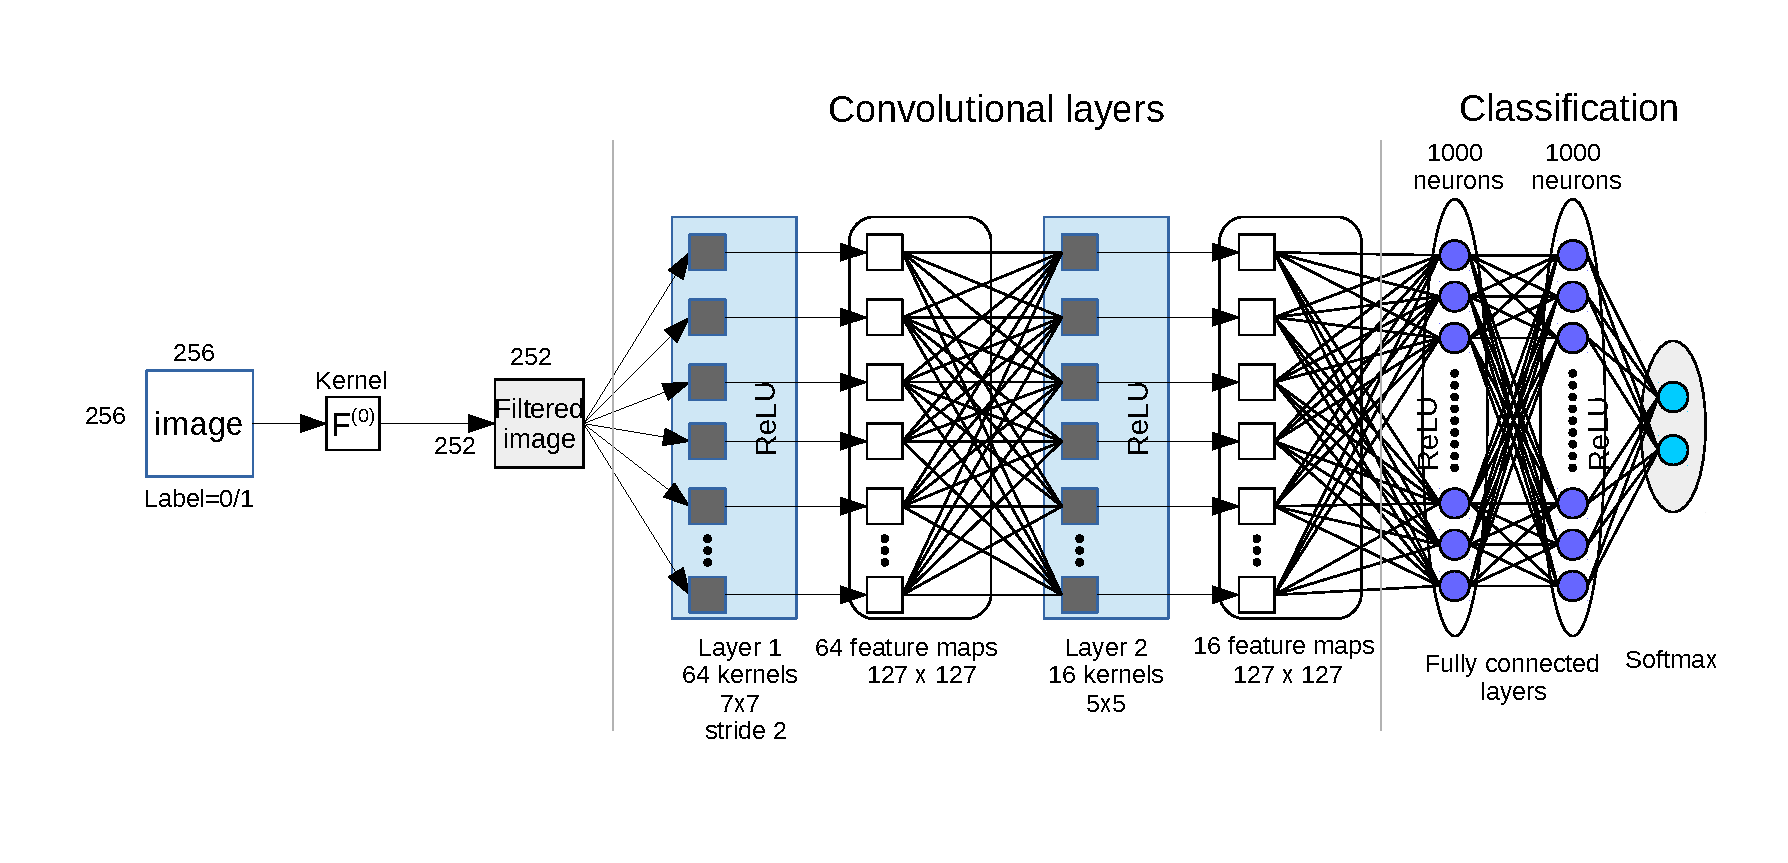
\includegraphics[width=0.70\textwidth]{Figures/CNN_eng.eps}
	\end{center}

	\caption{An example of Convolutional Neural Network (CNN) architecture with a first fixed Kernel to pre-processing the input image, two convolutional layers to manage image autocorrelation, two fully connected layers to prepare the prediction step and, finally, a SoftMax layer to perform the final classification. \label{cnn_example}}
\end{figure}

\subsection{Deep Learning in Heterogeneous and Incomplete Data}
In 2015 I started to investigate Deep Learning methods and, still in the same year, I started the co-supervision with Dr. Marc Chaumont (LIRMM) and Dr. Gerard Subsol (LIRMM) of the PhD Thesis of M. Lionel Pibre on the "Detection of urban objects from heterogenous remote sensing data sources".
This work will be devoted to the use of deep learning techniques on heterogeneous remote sensing data to detect objects ( i.e. trees) in urban areas. As an objective, we would overpass some limitations of standard supervised approaches on heterogenous multi source data.

Standard classification algorithms need a training phase before being employed on new unseen examples (test data). A challenge in this field can be the development of new deep learning architectures to manage heterogeneous data coming from different sensors (optical sensor, satellite images, drone images, Radar images, etc...)  in a setting where training and test data cannot fit the same format and, commonly, the test set is poorer (in terms of information) than the training set. 
In this case we can exploit previous approaches proposed in the field of deep and representational learning~\cite{LeCun15,BengioCV13} in order to obtain some intermediate representation coping with partial information. Such intermediate representation can be obtained employing some kind of autoencoder tool~\cite{VincentLLBM10}.
Successively, the deep learning system can be trained on such intermediate representation and, once a new unseen example is available, first of all it will be transformed employing an autoencoder and then the transformed instance can be the input of the predictive model to get the final classification.

During the preliminary experiments we conducted, we observed that the results are heavily influenced by the type of activation function employed in a particular layer of the CNN. Studying some kind of adaptive way to choose which activation function could be used in which layer can be useful in general. For instance, instead to use a single activation functions~\cite{BengioCV13} (ReLU, eLU, etc...) for each layer, maybe a weighted linear (or not linear) combination of such functions can allow the network to automatically learn which one is more suitable at which point of the architecture.
All these perspectives can be developed considering as an application scenario the analysis of remote sensing images where, only in the last two years, deep learning approaches started getting increasing attention~\cite{LuusSBM15,MarmanisDES16}.


\subsection{Deep Learning for image data archives}
As well underlined by~\cite{LeCun15}, one of the possible future directions of deep learning is the use of such models in an unsupervised way. Recently, due to the rapid evolution of satellite system, large-scale remote sensing image data archives are more and more available and they need practical tools to organize and retrieve such information. An exhaustive search through linear scan over such archives is really time-consuming and not practically reasonable in real world applications. Recently, \cite{DemirB16} proposes an hashing-based scalable remote sensing image search systems to overcome this problem employing kernel methods to hash such images. An interesting point to investigate could be the use of Deep Learning architecture in order to compress remote sensing satellite images performing some kind of Local Sensitivity Hashing~\cite{GionisIM99} to speed up the search and retrieval process. Such hashing can be successively indexed by some tree structure and the index can support approximate similarity queries. Leveraging the ability of CNN to model spatial auto-correlation, the obtained compressed representation can implicitly incorporate spatial information.
The encoding supplied by the Deep learning strategies can be learnt in both unsupervised or (partially) supervised ways in order to supply a more efficient image search engine.
Combining Deep Models (with a representational purpose) with information retrieval and database techniques to manage and query archive of remote sensing satellite images can be an interesting field of research. In the past, examples in which machine learning techniques are employed to optimize and ameliorate database and information retrieval systems have already pointed out their usefulness~\cite{AkdereCRUZ11,AkdereCRUZ12}.

\subsection{Mixing Convolutional and Recurrent Neural Networks}
Among the perspectives in the Deep Learning fields, listed by~\cite{LeCun15}, the improvement of current deep methods to deal with dynamic systems or sequential inputs will be one point to address in the near future. The particular neural architecture devoted to manage sequential and temporal information is called Recurrent Neural Network (RNN). 
RNNs are valuable tools that started to demonstrate their interest to classify and compress sequential data~\cite{GreffSKSS15}. 
RNNs manage an input sequence one element at a time, maintaining in their hidden units a ‘state vector’. Such a vector implicitly represents the information about the history of all the past elements of the sequence. RNNs, once unfolded considering the time dimensions, can be seen as a very deep feedforward networks in which all the layers share the same weights.
One of the major problem of such architecture was the training phase over many time steps, in which, the network can typically explode. Recent advances in the domain of RNNs proposed techniques such as Long Short-Term Memory (LSTM) and its variants~\cite{GreffSKSS15}. In order to deal with the problem to remember too long events, such approaches have hidden states employed as memory. The role of these hidden states is to propagate the same information from a time stamp to the next one. The improvement of such architectures is related to the ability to learn when such memories can be re-initialized or not.

In the context of time series of satellite images, as previously discussed, both spatial and temporal aspects play an important role. Such characteristics are crucial to understand the underlying behavior for both classification and summarization purposes. CNNs show impressive performance for image analysis while RNNs demonstrate their ability to model temporal data. A possible research direction can be the combination of these two models in the context of remote sensing data. What can be proposed is an hybrid architecture able to learn, at the same time, convolutional filters that are related to particular portions of the input sequences exploiting the ability of RNNs to model recurrent phenomena.

\section{Conclusion}
The first law of geography tells us that “everything is related to everything else but nearby things are more related than distant things”. Such a characteristic is also known as the spatial autocorrelation. Therefore, the widely used i.i.d. assumption in data mining is too strong when analyzing spatial data. New methods and modeling techniques are needed to tackle the spatial heterogeneity and the spatial relationships (such as topological relationships, directional relationships, etc.), which are unique to spatial data. Spatio-temporal data are further temporally dynamic, which requires explicit or implicit modeling of the spatio-temporal autocorrelation and constraints to achieve good prediction performance\footnote{\url{http://researcher.watson.ibm.com/researcher/view_group.php?id=4152}}.
This is why, in the past, I concentrated my effort on spatio-temporal data and this is also why I would continue, in a near future, to investigate new data mining and machine learning approaches for Spatio-Temporal data with more emphasis on the spatial component.  %for instance, the perspective I sketched before in this chapter.

Le me conclude by stating the following observation: research is an active process that involves as well junior as senior researchers and as well PhD as PostDoc. From my reduced experience, research is a collective activity in which people collaborate with each others sharing experiences and new points of view about the same task. My past research was influenced by  people I worked with during visiting periods, conferences, and project collaborations. Likewise, my future research will be influenced by new people I will meet in this never ending trip that is research.


